\documentclass[twoside,colorbacktitle,accentcolor=tud2b]{tudexercise}
\usepackage{syntax}
\usepackage{listings}
\usepackage{tikz}
\usetikzlibrary{trees}
\usepackage{ngerman}
\usepackage{amsmath}
\newcommand{\unit}[1]{{\rm\,#1}}
\renewcommand{\syntleft}{} 
\renewcommand{\syntright}{}
\title{\textsf{Einführung in den \linebreak Compilerbau} \linebreak \small Doan Nam Long Vu, Van Khai Ngo, Sascha Hoffman}
\subtitle{Wintersemester 2019/2020}
\subsubtitle{Theorieblatt \arabic{section}}


\begin{document}
\setcounter{section}{1}
\maketitle
  \subsection{MAVL-Syntax}
  \begin{enumerate}
  	\item 
  	\subitem Subtracktion
  	\begin{grammar}
  	<"subExpr"> ::= "expr" "'-'" "expr"
  \end{grammar}
  \subitem Matrix-Transponierung
  \begin{grammar}
  	<"transposeExpr"> ::= "'~'"  "matrixExpr" 

	<"marixExpr"> ::= "'matrix'" 
	\alt "matrixExpr" "Operator" "matrixExpr"
	\alt "matrixExpr" "'*'" "(FLOAT|INT)"
	\alt  "(FLOAT|INT)" "'*'" "matrixExpr" 
	\alt "transposeExpr"

	<"Operator"> ::= "'+'|'-'|'#'" 
\end{grammar}
\subitem Subvektor-Operator
  \begin{grammar}
	<"subvektorExpr"> ::= ID "'{'""expr"':'"expr"':'"expr""'}'" 
\end{grammar}
 
  \item primitive Typen
 \begin{grammar}
 	 <"primitiveType"> ::= "('float'|'bool'|'int')"
\end{grammar}

 \subitem Vektortypen
  \begin{grammar}
 	<"vectorType"> ::= "'vector'""'<'""('int'|'float')""'>'" "'[' expr ']'"
 	
 \end{grammar}

 \item  Rückgabebefehl
 \begin{grammar}
 	<"returnStmt"> ::= "'return'" "expr" "';'"
 \end{grammar}
 
 \subitem Variabledeklaration
 	\begin{grammar}
 	<"varDecl"> ::=   "'var'" "type ID" "';'"
 \end{grammar}

 \subitem Aufruf-Befehl, ohne Rückgabewert
  \begin{grammar}
  	<"callStmt"> ::= "ID"" '('(expr',')*expr')'" "';'"
  	\alt "ID" '(' ')' "';'"
  \end{grammar}
  
 \item Konstante Ausrücke
 
 \begin{grammar}
 	<"constExpr"> ::= "INT" | "constExpr" "Operator" "constExpr"
 	
 	<"Operator"> ::= "'+'|'-'|'*'|'/'|'^'"
 \end{grammar} 
  \end{enumerate}
\clearpage

  \subsection{AST$\,\to\,$MAVL}
    \begin{enumerate}
      \item MAVL-Code
      \begin{lstlisting}
      	if(tongle || r < s){
      		r = (r-s)/2;
      		val int d = s-r;
      		update(d,r);
      		}
   \end{lstlisting}
      \item MAVL-Code
      	\begin{lstlisting}
      	switch(k){
      		case -1:
      			r = 0;
      		default:
      			 r = k-1;      		
      	}
      	\end{lstlisting}
      
    \end{enumerate}
  \subsection{Ausdrücke}
    \begin{enumerate}
   \item \leavevmode\vadjust{\vspace{-\baselineskip}}\newline
   \begin{tikzpicture}[
   tlabel/.style={pos=5,right=-1pt,font=\footnotesize\color{black}},
   ]
   \node{And}
    [sibling distance=3cm]
  child{node{''q''}}
  child{node{Compare}
  		child{node{''a''}}
  		child{node{Subtraction}
  					child{node{''b''}}
  					child{node{''c''}}
  		}
  	}
; \end{tikzpicture}
   \item 
   Der Ausdruck aus a) ist syntaktish korrekt aber semantisch falsch.
   Laut Operantorpräzenden wird (b-c) zuerst berechnet und dann mit a vergleichen,
   aber (b-c) ist von Typ int und a ist von Typ bool, deshalb kann kein semantisch korrekte AST erstellt werden.
  \item \leavevmode\vadjust{\vspace{-\baselineskip}}\newline
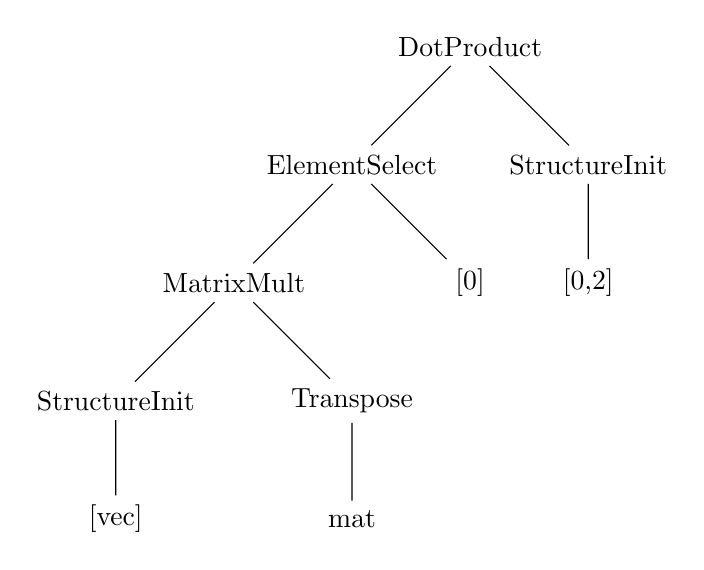
\begin{tikzpicture}
	\node{DotProduct}
	 [sibling distance=3cm]
	 child{node{ElementSelect}
	 	child{node{MatrixMult}
	 		child{node{StructureInit}
	 			child{node{[vec]}}
	 		}
	 		child{node{Transpose}
	 			child{node{mat}}
	 		}
	 	}
	 	child{node{[0]}}
}
child{node{StructureInit}
	child{node{[0,2]}}	
};
\end{tikzpicture}

\item Aus c) 

\[(\begin{pmatrix}
	5 & 6\\
\end{pmatrix}
\begin{pmatrix}
	1 & 2\\
	3 & 1\\
\end{pmatrix}^\top)
\begin{bmatrix}
0
\end{bmatrix}
.
\begin{pmatrix}
	0 & 2\\

\end{pmatrix}
\\
=(\begin{pmatrix}
5 & 6\\
\end{pmatrix}
\begin{pmatrix}
1 & 3\\
2 & 1\\
\end{pmatrix}^\top)
\begin{bmatrix}
0
\end{bmatrix}
.
\begin{pmatrix}
0 & 2\\

\end{pmatrix} \\
=
\begin{pmatrix}
17 & 21\\

\end{pmatrix}
\begin{bmatrix}
0
\end{bmatrix}
.
\begin{pmatrix}
0 & 2\\

\end{pmatrix} 
= 42
\]

$\Rightarrow$ 
Der Ausdruck aus Teilaufgabe c) liefert den Wert gleich 42.
\end{enumerate}
\end{document}
